\documentclass[12pt,oneside]{uhthesis}
\usepackage{subfigure}
\usepackage[ruled,lined,linesnumbered,titlenumbered,algochapter,spanish,onelanguage]{algorithm2e}
\usepackage{amsmath}
\usepackage{amssymb}
\usepackage{amsbsy}
\usepackage{caption,booktabs}
\captionsetup{ justification = centering }
%\usepackage{mathpazo}
\usepackage{float}
\setlength{\marginparwidth}{2cm}
\usepackage{todonotes}
\usepackage{listings}
\usepackage{xcolor}
\usepackage{multicol}
\usepackage{graphicx}

\floatstyle{plaintop}
\restylefloat{table}
\addbibresource{Bibliography.bib}
% \setlength{\parskip}{\baselineskip}%
\renewcommand{\tablename}{Tabla}
\renewcommand{\listalgorithmcfname}{Índice de Algoritmos}
%\dontprintsemicolon
\SetAlgoNoEnd

\definecolor{codegreen}{rgb}{0,0.6,0}
\definecolor{codegray}{rgb}{0.5,0.5,0.5}
\definecolor{codepurple}{rgb}{0.58,0,0.82}
\definecolor{backcolour}{rgb}{0.95,0.95,0.92}

\lstdefinestyle{mystyle}{
    backgroundcolor=\color{backcolour},   
    commentstyle=\color{codegreen},
    keywordstyle=\color{purple},
    numberstyle=\tiny\color{codegray},
    stringstyle=\color{codepurple},
    basicstyle=\ttfamily\footnotesize,
    breakatwhitespace=false,         
    breaklines=true,                 
    captionpos=b,                    
    keepspaces=true,                 
    numbers=left,                    
    numbersep=5pt,                  
    showspaces=false,                
    showstringspaces=false,
    showtabs=false,                  
    tabsize=4
}

\lstset{style=mystyle}

\title{Sintetizador de Voz en Español con Voces Cubanas}
\author{\\\vspace{0.25cm}Sandra Martos Llanes}
\advisor{\\\vspace{0.25cm}Lic. Katy Castillo Rosado\\\vspace{0.2cm}Dr.Cs. Flavio Reyes Díaz}
\degree{Licenciado en Ciencia de la Computación}
\faculty{Facultad de Matemática y Computación}
\date{Fecha\\\vspace{0.25cm}\href{https://github.com/username/repo}{github.com/username/repo}}
\logo{Graphics/uhlogo}
\makenomenclature

\renewcommand{\vec}[1]{\boldsymbol{#1}}
\newcommand{\diff}[1]{\ensuremath{\mathrm{d}#1}}
\newcommand{\me}[1]{\mathrm{e}^{#1}}
\newcommand{\pf}{\mathfrak{p}}
\newcommand{\qf}{\mathfrak{q}}
%\newcommand{\kf}{\mathfrak{k}}
\newcommand{\kt}{\mathtt{k}}
\newcommand{\mf}{\mathfrak{m}}
\newcommand{\hf}{\mathfrak{h}}
\newcommand{\fac}{\mathrm{fac}}
\newcommand{\maxx}[1]{\max\left\{ #1 \right\} }
\newcommand{\minn}[1]{\min\left\{ #1 \right\} }
\newcommand{\lldpcf}{1.25}
\newcommand{\nnorm}[1]{\left\lvert #1 \right\rvert }
\renewcommand{\lstlistingname}{Ejemplo de código}
\renewcommand{\lstlistlistingname}{Ejemplos de código}

\begin{document}

\frontmatter
\maketitle

\begin{dedication}
    Dedicación
\end{dedication}
\begin{acknowledgements}
	A mi madre por legarme su fortaleza y enseñarme en 22 años todo lo importante de la vida, a mi padre por apoyarme y estar siempre cerca de mí; y a ambos por ser mis ejemplos a seguir. 
	
	A mi hermano por su cariño, su cuidado y sus consejos, y a Heidy por su preocupación. 
	
	A mi abuela Mami por siempre velar por mí.
	
    A mis tíos: Edel, Julian, Nelson, Yuleika y Lucía por ser mis segundos padres. A mis primos Lauren, Lorena, Yoha, Ale y July por ser como mis hermanos, y especialmente a Yoha, por ser parte importante en la realización de esta tesis.
	 
	A todos mis amigos por hacer de estos 5 años los mejores, especialmente aquellos con los que he compartido risas, lágrimas, horas de estudio y momentos de diversión. Baby, Amalia, Ariel, Nadia, Luis y Jose, gracias por la oficina y \textit{for the good old days}.  
	
	A mis profesores, los que me inspiraron durante mi formación.
	
	A mis tutores por la confianza depositada. Flavio por su guía durante este proceso, y Katy por motivarme y ser parte de mi familia.
	
	A todos los que me ayudaron a alcanzar esta meta, muchísimas gracias.
	
	
	 
	
   
\end{acknowledgements}
\begin{opinion}
    Opiniones de los tutores
\end{opinion}
\begin{resumen}
Este Trabajo de Diploma muestra los resultados de la investigación realizada para encontrar un método de síntesis de voz, en español para adaptar a la voz cubana. La investigación se centra en diversas cuestiones. La primera, es el estado de la síntesis de voz mediante aprendizaje profundo en la actualidad, y la complejidad para poder generar una voz artificial con este método. Se eligen las herramientas para llevar a cabo esta tarea, así como los modelos Tacotron2 y VITS con el mismo fin, un sistema de dos etapas y un modelo de extremo a extremo respectivamente. Se construye una base de datos con un hablante cubano para cumplir con el requisito del acento cubano en el sistema de conversión de texto a voz que se persigue desarrollar. Se experimenta mediante entrenamientos y reentrenamientos de difentes variantes de los modelos antes mencionados, especialmente del modelo VITS, pues el modelo Tacotron2 arroja resultados desanlentadores desde las primeras etapas. Por último se realiza una evaluación de los resultados donde se concluye que la mayor importancia para el cumplimiento satisfactorio del objetivo principal, que es el desarrollo de un sintetizador de voz en español, adaptado a la voz cubana, está en los conjuntos de datos para el entrenamiento de modelos. 
\end{resumen}

\begin{abstract}
	This thesis shows the results of the research carried out to find a method of voice synthesis, in Spanish to adapt to Cuban accent. The research focuses on a variaty of issues. First, the recent studies on the field of text to speech synthesis using deep learning, and the complexity of being able to generate an artificial voice through this method. It was necesary the selection of tools to carry out this task, as well as DNN-based model such as Tacotron2 and VITS model: a two-stage and an end-to-end model respectively. A database with a Cuban speaker is built to meet the Cuban accent requirement in the aimed text-to-speech conversion system. There were experiments conducted through training and fine-tuninf of different variants of the previously mentioned models, especially the VITS model, since the Tacotron2 model yields discouraging results from early stages. Finally, an evaluation of the results is carried out, where it is concluded that the most important aspect for the satisfactory fulfillment of the main objective, which is the development of a voice synthesizer in Spanish, adapted to the Cuban voice, is in the data sets for the model training.
\end{abstract}
\tableofcontents
\listoffigures
% \listoftables
% \listofalgorithms
\lstlistoflistings

\mainmatter

\chapter*{Introducción}\label{chapter:introduction}
\addcontentsline{toc}{chapter}{Introducción}

La era de la informática conversacional está cambiando la forma en la que los usuarios interactuan con sus dispositivos: el Asistente de Google busca en Internet y lee las instrucciones sobre cómo preparar un pastel, Siri guía en la búsqueda de un lugar desconocido, las líneas automatizadas de servicio al cliente operan sin necesidad de esperas o botones. Uno de los primeros problemas que alguien se plantearía es la comunicación con los dispositivos, y es que no es posible determinar de qué forma va a
interactuar una persona con estos. Se pueden hacer aproximaciones y suposiciones, pero cada persona puede decidir operar de una forma diferente, y sería imposible que un actor de voz grabase infinitas respuestas a las ramas de conversación que pueden surgir de una simple pregunta. En este punto entra la síntesis de voz, si en vez de unas grabaciones, el dispositivo pudiese sintetizar una voz humana, podría responder y hablar con la persona, entablando una especie de conversación.\\

%todo esto es posible gracias a la tecnología digital llamada texto a voz o TTS por sus siglas en inglés. \\


La síntesis de voz es la producción artificial del habla humana. Se han diseñado diferentes sistemas para este propósito, llamados sintetizadores de voz y pueden ser implementados tanto en hardware como en software. Un sistema de conversión texto a voz (TTS, por sus siglas en inglés, \textit{text to speech}) o sintetizador de voz, toma como entrada, texto y produce como salida voz audible. Este sistema de conversión, se compone básicamente por dos componentes: un modelo que predice generalmente en forma de espectograma, la mejor pronunciación posible de cualquier texto dado, y un codificador de voz que, a partir del espectograma anterior produce ondas sonoras de voz.\\

El texto a voz es un campo particularmente disciplinario, que requiere un conocimiento
detallado en una variedad de ciencias. Si se quisiera construir un sistema TTS desde cero, se tendrían que estudiar los siguientes temas:

\begin{itemize}
	\item Lingüística, el estudio científico del lenguaje. Para sintetizar un habla coherente, los sistemas TTS necesitan reconocer cómo un hablante humano pronuncia el lenguaje escrito; esto requiere conocimientos de lingüística hasta el nivel del fonema: las unidades de sonido que combinadas producen el habla, como el sonido /t/ en tierra. Para lograr un TTS verdaderamente realista, el sistema también necesita predecir la prosodia apropiada,que incluye elementos del habla más allá del fonema, como acentos, pausas y entonación.
	
	\item Procesamiento de señales de audio, creación y manipulación de representaciones digitales de sonido. Las señales de audio (habla) son representaciones electrónicas de ondas sonoras. La señal de voz se representa digitalmente como una secuencia de números. En el contexto de TTS se utilizan diferentes representaciones de características que describen la señal del habla, lo que hace posible entrenar diversos modelos para generar una nueva voz.
	
	\item Inteligencia artificial, especialmente aprendizaje profundo, un tipo de aprendizaje automático que utiliza una arquitectura informática llamanda red neuronal profunda o DNN por sus siglas en inglés. Una red neuronal es un modelo computacional inspirado en el cerebro humano. Está formado por redes complejas de procesadores, cada uno de los cuales realiza una serie de operaciones antes de enviar su salida a otro procesador. Una DNN capacitada aprende la mejor vía de procesamiento para lograr resultados precisos. Este modelo tiene una gran potencia informática, lo que lo hace ideal para manejar la gran cantidad de variables necesarias para la síntesis de voz de alta calidad.
\end{itemize}

\subsubsection*{Tipos de tecnologías TTS}

Hasta la actualidad se han desarrollado variadas tecnologías TTS, las cuales operan de maneras distintas. Entre las más dominantes se encuentran: 

\begin{enumerate}
	\item  Síntesis de formantes y síntesis articulatoria: \\Los primeros sistemas TTS empleaban tecnologías basadas en reglas, como la síntesis de formantes y la síntesis articulatoria, que logró un resultado similar a través de estrategias ligeramente diferentes. A partir de una grabación realizada a un hablante, se extrajeron características acústicas de este: formantes, cualidades definitorias de los sonidos del habla, en síntesis de formantes; y forma de articulación (nasal, oclusiva,vocal,etc.) en síntesis articulatoria. Luego, se programarían reglas que recrearan estos parámetros con una señal de audio digital. Este TTS era bastante robótico; y estos enfoques necesariamente abstraen gran parte de la variación que se encontrará en el habla humana, cosas como la variación de tono, porque solo permiten a los programadores escribir reglas para unos pocos parámetros a la vez.
	
	\item Síntesis de difonos: \\ El próximo gran desarrollo en el campo TTS se llama síntesis de difonos, se inició en la década de 1970 y todavía era de uso popular durante los últimos años del siglo XX. La síntesis de difonos crea  un habla de máquina mediante la combinación de difonos, combinaciones de fonemas de una sola unidad, y las transiciones de un fonema al siguiente; es decir, no solo la /t/ en la palabra tierra sino la /t/ más la mitad del siguiente sonido /i/. 
	
	La tecnología TTS de síntesis de difonos incluye también modelos que predicen la duración y el tono de cada difono para la entrada dada. Estos dos sistemas se superponen el uno sobre el otro, primero conecta las señales de difono y luego procesa la señal para corregir el tono y la duración. El resultado es un discurso  sintético con un sonido más natural que el que crea la síntesis de formantes, pero aún está lejos de ser perfecto, y tiene pocas ventajas sobre cualquier otro acercamiento. 
	
	\item Síntesis de selección de unidades: \\ La síntesis de selección de unidades constituye un enfoque ideal para los motores TTS de bajo impacto en la actualidad. Cuando la síntesis de difonos añadió duración y el tono apropiado a través de un segundo sistema de procesamiento, la síntesis de selección de unidad omite ese paso: se inicia con una gran base de datos grabados del habla, alrededor de 20 horas o más, y se seleccionan los fragmentos de sonido que ya tienen la duración y el tono deseado. La síntesis de selección de unidades proporciona un habla similar a la humana sin mucha modificación de la señal, pero sigue siendo identificablemente artificial. Probablemente el audio de salida de la mejor selección de unidades, sea indistinguible de las voces humanas reales, especialmente en contextos con sistemas TTS. Sin embargo, un mayor naturalidad requiere de bases de datos de selección de unidades muy grandes, en algunos sistemas llegando a ser de gigabytes de datos grabados, representando docenas de horas de voz. 
	
	\item Síntesis neuronal: \\ La tecnología de las redes neuronales profundas es la que impulsa los avances actuales en el campo TTS, y es clave para la obtención de resultados mucho más realistas. Al igual que sus predecesores, el TTS neuronal comienza con grabaciones de voz; la otra entrada es texto, el guión escrito que su locutor de origen utilizó para crear esas grabaciones. Esas entradas alimentan una red neuronal profunda y se aprende el mejor mapeo posible entre un bit de texto y las características acústicas asociadas. 
	
	Una vez que el modelo esté entrenado, podrá predecir sonido realista para nuevos textos: con un modelo TTS neuronal entrenado, junto con un codificador de voz entrenado con los mismos datos, el sistema puede producir un habla que es notablemente similar a la del locutor de origen cuando se expone a prácticamente cualquier texto nuevo. Esa similitud entre la fuente y la salida	es la razón por la que el TTS neuronal a veces se denomina “clonación de voz”.
	
	Hay todo un grupo de métodos de procesamiento de señales que pueden ser utilizados para alterar la voz sintética resultante y no se asemeje al locutor fuente. En la actualidad, las principales investigaciones se enfocan en lograr voces TTS que hablan con expresión emocional, voces únicas en varios idiomas y una calidad de audio cada vez más realista.
\end{enumerate}

Entre las aplicaciones que hacen uso del TTS, se encuentran:

\begin{itemize}
	\item Sistemas de respuesta de voz interactiva conversacional (IVR), como en los centros de llamadas de servicio al cliente.
	
	\item Aplicaciones de comercio de voz, como comprar en un dispositivo Amazon Alexa.
	\item Herramientas de navegación y guía por voz, como aplicaciones de mapas GPS.
	\item Dispositivos domésticos inteligentes y otras herramientas de Internet de las cosas (IoT) habilitadas por voz.
	\item Asistentes virtuales independientes, como Siri de Apple.
	\item Soluciones de publicidad y marketing experiencial, como anuncios de voz interactivos en servicios de transmisión de música.
	\item Desarrollo de videojuegos.
	\item Videos de marketing y formación de la empresa que permiten a los creadores cambiar las	voces en off sin identificar al locutor.
\end{itemize}

\section*{Problemática}
Existe un conjunto de sistemas TTS que se enmarcan bajo una licencia de software libre:
\begin{itemize}
	\item Festival y Festvox
	\item Plataforma MaryTTS
	\item Sistema TTS
	\item SV2TTS
	\item Mozilla-TTS
	\item COQUI -TTS
\end{itemize}


A partir del estudio parcial de las plataformas de código abierto utilizadas para el desarrollo de conversores de texto a voz, fue posible comprobar que la mayoría se encuentran basadas en la síntesis neuronal teniendo en cuenta que alcanza mejores resultados. Estas plataformas brindan modelos previamente entrenados para idiomas específicos como inglés, francés, alemán, etc. Muy pocas presentan un modelo en español, y las que lo hacen solo poseen uno, con acento de voz española o voz neutra.\\

DATYS, es una empresa de desarrollo de software, que como parte de sus soluciones requiere un sintetizador de voz en español con acento propio de nuestro país; esto formará parte de un proyecto que consiste en el desarrollo del primer asistente virtual cubano. 

\section*{Objetivo}

\subsection*{Objetivo General}

Desarrollar un sintetizador de texto a voz con voces cubanas.

\subsection*{Objetivos específicos}
\begin{enumerate}
	\item Analizar en profundidad los métodos y plataformas existentes para la síntesis de voz, principalmente las que trabajan sobre la síntesis neuronal, y seleccionar el más adecuado a utilizar para las aplicaciones de DATYS.
	\item Diseñar y conformar una base de datos en español, con con voces cubanas para el entrenamiento de los modelos y muestras de voz que se desea generar.
	\item Reentrenar el modelo basado en síntesis neuronal seleccionado, para su ajuste al estilo de voz cubana.
	\item Evaluar el modelo entrenado.
\end{enumerate}
\chapter{Estado del Arte}\label{chapter:state-of-the-art}

Las redes neuronales han sido las encargadas de los avances actuales en el campo TTS, por tanto esta será la línea seguida en la investigación. \\


Coqui TTS[\cite{coqui-doc}] es una biblioteca para la generación avanzada de texto a voz. Se basa en las últimas investigaciones y se diseñó para lograr el mejor equilibrio entre la facilidad de entrenamiento, la velocidad y la calidad. Coqui viene con modelos preentrenados, herramientas para medir la calidad del conjunto de datos y ya se utiliza en más de 20 idiomas para productos y proyectos de investigación.


Para lograr la transformación de texto a voz, Coqui sigue dos enfoques distintos. El primero es un sistema de dos estapas: una combinación de dos modelos, uno para convertir de texto a espectograma de mel, y luego otro de espectograma a onda sonora; y el segundo es un modelo de extremo a extremo.  

\section{Sistemas de dos etapas}

El paradigma predominante en la conversión de texto a voz es la síntesis en dos etapas: primero, producir espectrogramas a escala de mel a partir del texto y, luego, las ondas de sonido reales con un modelo de codificador de voz(VoCoder). La representación acústica de bajo nivel: espectograma de mel, es la utilizada como nexo entre las dos componentes.


\subsection{Modelos TTS}

\subsubsection{FastSpeech}

FastSpeech, una novedosa red de avance basada en Transformer para generar espectrogramas de mel en paralelo para TTS; toma como entrada una secuencia de texto(fonema) y genera espectrogramas de mel de forma no autorregresiva. Adopta una red feed-forward basada en la autoatención en Transformer y convolución de 1D. 

%Dado que una secuencia de espectrograma mel es mucho más larga que su correspondiente secuencia de fonemas, para resolver el problema de la falta de coincidencia de longitud entre las dos secuencias, FastSpeech adopta un regulador de longitud que aumenta la muestra de la secuencia de fonemas de acuerdo con la duración del fonema (es decir, el número de espectrogramas mel a los que corresponde cada fonema) para que coincida con la longitud de la secuencia del espectrograma mel. El regulador se basa en un predictor de duración de fonemas, que predice la duración de cada fonema. 
%En lugar de utilizar la arquitectura basada en codificador-atención-decodificador adoptada por la mayoría de las generaciones autorregresivas y no autorregresivas basadas en secuencia a secuencia.

El modelo resuelve problemas existentes en otros modelos TTS de la siguiente forma:

\begin{itemize}
	\item A través de la generación de espectrogramas de mel paralelos, FastSpeech acelera enormemente el proceso de síntesis.
	\item El predictor de duración de fonemas asegura alineaciones estrictas entre un fonema y sus espectrogramas, lo que es muy diferente de las alineaciones de atención automáticas y suaves en los modelos autorregresivos. Por lo tanto, FastSpeech evita los problemas de propagación de errores y alineaciones de atención incorrectas, lo que reduce la proporción de palabras omitidas y palabras repetidas.
	\item El regulador de longitud puede ajustar fácilmente la velocidad de la voz alargando o acortando la duración del fonema para determinar la duración de los espectrogramas de mel generados, y también puede controlar parte de la prosodia añadiendo pausas entre fonemas adyacentes.
\end{itemize}


\textbf{Arquitectura}\\

Feed-Forward Transformer: \\
La arquitectura para Fast Speech es una estructura de avance basada en la autoatención en Transformer y la convolución de 1D; se nombra esta estructura como Feed-Forward Transformer (FFT). Feed-Forward Transformer apila múltiples bloques FFT para la transformación de fonema a espectrograma de mel, con $N$ bloques en el lado del fonema y $N$ bloques en el lado del espectrograma de mel, con un regulador de longitud en el medio para cerrar la brecha de longitud entre el fonema y la secuencia del espectrograma de mel. Cada bloque FFT consta de una red convolucional de 1D y de autoatención. La red de autoatención consiste en una atención de múltiples cabezas para extraer la información de posición cruzada. \\ %Las conexiones residuales, la normalización de capas y el abandono(drop-out) se agregan después de la red de autoatención y la red convolucional 1D, respectivamente.\\

Regulador de longitud: \\
El regulador de longitud se utiliza para resolver el problema de la discordancia de longitud entre el fonema y la secuencia del espectrograma en el transformador de avance, así como para controlar la velocidad de la voz y parte de la prosodia. La longitud de una secuencia de fonemas suele ser menor que la de su secuencia de espectrograma de mel, y cada fonema corresponde a varios espectrogramas de mel. \\

Predictor de duración: \\
La predicción de la duración de los fonemas es importante para el regulador de longitud.
El predictor consta de una red convolucional de 1D de 2 capas con activación ReLU, cada una seguida de la normalización de la capa y la capa de exclusión, y una capa lineal adicional para generar un escalar, que es exactamente la duración prevista del fonema.\\

\textbf{Experimentación}\\

El entrenamiento de FastSpeech y de todos los modelos TTS se realiza sobre un conjunto de datos que contiene clips de audios con sus correspondientes transcripciones de texto. Específicamente para FastSpeech, se divide al azar el conjunto de datos en 3 conjuntos: muestras para entrenamiento, muestras para validación y muestras para las pruebas. \\


El modelo FastSpeech puede casi coincidir con el modelo autoregresivo Transformer TTS en términos de calidad de voz, acel
era la generación de espectrograma mel por 270x y la síntesis de voz de extremo a extremo por 38x, casi se elimina el problema de saltar y repetir palabras, y puede ajustar la velocidad de voz (0.5x-1.5x) sin problemas[\cite{ren2019fastspeech}].


\subsubsection{FastPitch}
FastPitch es un modelo TTS feed-forward completamente paralelo basado en FastSpeech, condicionado por contornos de frecuencia fundamentales. El modelo predice contornos de tono durante la inferencia. Al alterar estas predicciones, el discurso generado puede ser más expresivo, coincidir mejor con la semántica del enunciado y, al final, ser más atractivo para el oyente.

Los modelos paralelos pueden sintetizar órdenes de magnitud de espectrogramas de mel más rápido que los autorregresivos, ya sea basándose en alineaciones externas o alineándose ellos mismos. El condicionamiento en la frecuencia fundamental también mejora la convergencia y elimina la necesidad de destilar el conocimiento de los objetivos del espectrograma de mel utilizados en FastSpeech.\\

\textbf{Arquitectura}\\

Se basa en FastSpeech y se compone principalmente de dos pilas de transformadores alimentados hacia adelante, feed-forward(FFTr) . El primero opera en la resolución de los tokens de entrada, el segundo en la resolución de los cuadros de salida.
La primera pila de FFTr produce la representación oculta $h$. La representación oculta, se usa para hacer predicciones sobre la duración y el tono promedio de cada caracter con una red neuronal convolucional de 1D.  A continuación, el tono se proyecta para que coincida con la dimensionalidad de la representación oculta y se suma a $h$. La suma se muestrea discretamente y se pasa a la salida FFTr, que produce la secuencia de espectrograma mel de salida[\cite{lancucki2021fastpitch}].\\

\textbf{Experimentación} \\
Para el entrenamiento y la experimentación los parámetros del modelo siguen principalmente FastSpeech.


\subsubsection{Tacotron}

Tacotron es un modelo TTS de tipo secuencia a secuencia con un paradigma de atención. Este modelo toma caracteres como entrada y devuelve un espectograma sin procesar usando técnicas para mejorar un modelo \textit{vanilla seq2seq}. Dado un par <texto,audio>, Tacotron puede ser entrenado desde cero con una inicialización aleatoria, y no requiere alineación a nivel de fonema.\\

\textbf{Arquitectura} \\

La columna vertebral de Tacotron es un modelo seq2seq con atención, que toma caracteres como entrada, y devuelve el correspondiente espectograma sin procesar, para luego pasarlo al modelo o algoritmo que sinteiza la voz. En el centro de todo esto se encuentra un codificador,un decodificador basado en atención y una red de post procesamiento.\\

Tacotron se basa en cuadros, o frames en inglés, por lo que la inferencia es sustancialmente más rápida que los métodos autorregresivos a nivel de muestra. A diferencia de otros trabajos más antiguos, Tacotron no necesita características lingüísticas diseñadas a mano ni componentes complejos como un alineador de Modelo Markov oculto(HMM). Este modelo realiza una
normalización de texto simple[\cite{wang2017tacotron}].


\subsubsection{Tacotron 2}

Tacotron 2 es similar al anteriormente mencionado Tacotron; es una red recurrente de predicción de características, de tipo secuencia a secuencia con atención, que mapea incrustaciones(embeddings) de caracteres en espectrogramas a escala de mel. 

Un espectrograma de frecuencia de mel está relacionado con el espectograma de frecuencia lineal, es decir, la magnitud de la transformada de Fourier de tiempo corto (STFT). Se obtiene aplicando una transformada no lineal al eje de frecuencia de la STFT, inspirado en respuestas calificadas por el sistema auditivo humano, y resume el contenido de frecuencia con menos dimensiones.

El uso de una escala de frecuencia auditiva de este tipo tiene el efecto de enfatizar detalles en frecuencias más bajas, que son fundamentales para la inteligibilidad del habla, al mismo tiempo que se resta importancia a los detalles de alta frecuencia, que están dominados por ráfagas de ruido y generalmente no necesitan ser modelados con alta fidelidad. Debido a estas propiedades, las características derivadas de la escala de mel se han utilizado como representación base para el reconocimiento de voz durante muchas décadas. 

Para Tacotron2 los espectrogramas de mel se calculan a través de un transformada de Fourier de tiempo corto (STFT) utilizando un tamaño de cuadro de 50 ms, 12,5 ms de salto de cuadro y una función de ventana de Hann. Se tranforma la magnitud de la STFT a la escala de mel usando un banco de filtros de 80 canales mel que abarca de 125 Hz a 7,6 kHz, seguido de una compresión de registro de rango dinámico. Antes de la compresión de registros, las magnitudes de salida del banco de filtros se recortan a un valor mínimo de 0,01 para limitar el rango dinámico en el dominio logarítmico.[\cite{shen2018natural}] \\

La red del modelo en cuestión está compuesta por un codificador y un decodificador con atención. El codificador convierte una secuencia de caracteres en una representación oculta que alimenta al decodificador para predecir un espectrograma.\\  

Los caracteres de entrada se representan utilizando una incrustación de caracteres 512-dimensional, que se pasan a través de una pila de 3 capas convolucionales, cada una de las cuales contiene 512 filtros con organización 5 × 1, es decir, donde cada filtro abarca 5 caracteres, seguido de la normalización por lotes y activaciones de ReLU[\cite{shen2018natural}]. Como en Tacotron, estas capas convolucionales modelan el contexto a largo plazo en la secuencia de caracteres de entrada. La salida de la capa convolucional final se pasa a una sola capa bidireccional LSTM que contiene 512 unidades (256 en cada dirección) para generar las características codificadas.



La salida del codificador es consumida por una red de atención que resume la secuencia codificada completa como un vector de contexto de longitud fija para cada paso de salida del decodificador. Se usa la atención sensible a la ubicación de [\cite{chorowski2015attention}], que extiende el mecanismo de atención aditiva [\cite{bahdanau2014neural}] para usar pesos de atención acumulativos de anteriores pasos de tiempo del decodificador como una funcionalidad adicional. Esto anima al modelo a seguir adelante consistentemente a través de la entrada, mitigando los posibles modos de falla donde algunas subsecuencias son repetidas o ignoradas por el decodificador.
Las probabilidades de atención se calculan después de proyectar las entradas y funciones de localización a representaciones ocultas de 128 dimensiones. Las funcionalidades de localización se calculan utilizando 32 filtros de convolución 1-D de longitud 31[\cite{shen2018natural}]. \\

El decodificador es una red neuronal autorregresiva recurrente que predice un espectrograma de mel a partir de la secuencia de entrada codificada un fotograma a la vez. La predicción del paso de tiempo anterior es primero pasado a través de una pequeña red previa que contiene 2 capas completamente conectadas de 256 unidades ReLU ocultas. La pre-red actuando como un cuello de botella de información es esencial para el aprendizaje de la atención.

La salida de la pre-red y el vector de contexto de atención se concatenan y pasan a través de una pila de 2 capas \textit{Long Short-Term Memory(LSTM)} unidireccionales con 1024 unidades. La concatenación de la salida LSTM y el vector de contexto de atención se proyecta a través de una transformación lineal para predecir el cuadro de espectrograma objetivo. Finalmente, se pasa el espectrograma de mel predicho a través de una post-red convolucional de 5 capas que predice un residuo a agregar a la predicción para mejorar la reconstrucción general. Cada capa post-net está compuesta por 512 filtros con forma 5×1 con lote normalización, seguida de activaciones de tanh en todas las capas excepto en la final[\cite{shen2018natural}].\\


En paralelo a la predicción de cuadros de espectrograma, la concatenación de
salida del decodificador LSTM y el contexto de atención se proyectan a un escalar y pasa a través de una activación sigmoidea para predecir la probabilidad de que la secuencia de salida se haya completado. La predicción de este ``token de parada'' se usa durante la inferencia para permitir que el modelo determine dinámicamente cuándo terminar la generación en lugar de generar siempre por una duración fija. Específicamente, la generación se completa en el primer fotograma para el que esta probabilidad supera un umbral de 0,5.\\

Las capas convolucionales en la red se regularizan usando abandono(dropout) con probabilidad 0.5, y las capas LSTM son regularizadas usando desconexión(zoneout) con probabilidad 0.1. Para introducir la variación de salida en tiempo de inferencia, se aplica dropout con probabilidad 0.5 solo a capas en la pre-red del decodificador autorregresivo[\cite{shen2018natural}].


En contraste con el Tacotron original, este modelo utiliza una construcción más simple, usando LSTM vainilla y capas convolucionales en el codificador y decodificador en lugar de pilas CBHG y capas recurrentes GRU. No se usa un "factor de reducción", es decir, cada paso del decodificador corresponde a un único cuadro de espectrograma.

Este sistema puede ser entrenado directamente desde un conjunto de datos sin depender de una compleja ingeniería de características, y logra calidad de sonido de última generación cercana a la del habla humana natural. Los resultados de Tacotron 2, constituyen un paso de avance sobre Tacotron y otros sistemas previos, sin embargo dejan aún espacio para mejoras. 


\subsection{VoCoders}
  Los VoCoders neuronales basados en redes neuronales profundas pueden generar voces similares a las humanas, en lugar de utilizar las tradicionales
  métodos que contienen artefactos audibles[\cite{griffin1984signal}][\cite{kawahara1999restructuring}][\cite{morise2016world}]. 
  
  La línea principal de la investigación se basa en los modelos TTS, como los antes expuestos, sin embargo como no es posible sintetizar voz sin un VoCoder, y luego de varias pruebas realizadas, se concluye que los más adecuados para el objetivo principal son los siguientes:

\subsubsection{UnivNet}
La mayoría de los codificadores de voz neuronales emplean espectrogramas de mel de banda limitada para generar formas de onda. UnivNet, es un codificador neural de voz que sintetiza formas de onda de alta fidelidad en tiempo real. 

Usando espectrogramas de mel de banda completa como entrada, se espera generar señales de alta resolución agregando un discriminador que emplea espectrogramas de múltiples resoluciones como entrada. En una evaluación de un conjunto de datos que contiene información sobre cientos de ponentes, UnivNet obtuvo los mejores resultados positivos, objetivos y subjetivos,  entre los modelos que competían. Estos resultados, incluida la mejor puntuación subjetiva en la conversión texto a voz, demuestran el potencial para una rápida adaptación a nuevos hablantes sin necesidad de entrenamiento desde cero[\cite{jang2021univnet}].

\subsubsection{WaveGrad}

WaveGrad es un modelo condicional para la generación de formas de onda que estima los gradientes de la densidad de datos. El modelo se basa en trabajos previos sobre emparejamiento de puntuaciones y modelos probabilísticos de difusión. Parte de una señal Gaussiana de ruido blanco e iterativamente refina la señal a través de un muestreador basado en gradientes, condicionado en el espectrograma de mel. WaveGrad ofrece una forma natural de intercambiar velocidad de referencia por calidad de la muestra ajustando el número de pasos de refinamiento, y cierra la brecha entre los modelos autorregresivos y no autorregresivos en términos de calidad de audio. El modelo puede generar muestras de audio de alta fidelidad usando como tan solo seis iteraciones. Los experimentos revelan que WaveGrad genera señales de audio de alta fidelidad, superando las líneas de base adversariales no autorregresivas y emparejando un fuertemente la línea de base autorregresiva basada en la probabilidad, utilizando menos operaciones secuenciales[\cite{chen2020wavegrad}].


\section{Modelos de extremo a extremo}
\subsection{VITS}

\textit{Variational Inference with adversarial learning for end-to-end Text-to-Speech (VITS)} es un método TTS de extremo a extremo en paralelo. Usando un Autocodificador Variacional se conectan los dos módulos de sistemas TTS: modelo acústico y VoCoder, a través de variables latentes para permitir el aprendizaje de extremo a extremo. 

Para mejorar el poder expresivo del método con el fin de sintetizar formas de onda de voz de alta calidad, se aplican flujos de normalización a la distribución condicional previa y entrenamiento adversarial en el dominio de formas de ondas.

El modelo VITS se describe principalmente en tres etapas: una formulación condicional de Autocodificador variacional; estimación de alineación derivada de la inferencia variacional; y entrenamiento adversarial para mejorar la calidad de la síntesis[\cite{kim2021conditional}].

(***No se si explicar cada parte)



Luego de un proceso de entrenamiento, experimentación y comparación con sistemas de dos etapas, utilizando los modelos preentrenados Tacotron2 y Glow-TTS como modelos de primer escenario e HiFi-GAN como modelo de segundo escenario, se comprueba que VITS obtiene un habla que suena más natural. Una evaluación humana subjetiva (puntuación de opinión media, o MOS) en LJ Speech, un conjunto de datos de un solo hablante, muestra que el modelo supera a los mejores sistemas TTS disponibles públicamente y logra un MOS comparable a la realidad del terreno.

Ha mostrado la capacidad de ampliarse a la síntesis de voz de múltiples hablantes, generando un discurso con diversos tonos y ritmos de acuerdo a diferentes identidades de hablantes. Esto demuestra que aprende y expresa varias características del habla en un contexto de extremo a extremo.



%Nuestro método adopta la inferencia variacional aumentada con flujos de normalización y un proceso de entrenamiento contradictorio, que mejora el poder expresivo del modelado generativo. También proponemos un predictor de duración estocástico para sintetizar el habla con diversos ritmos a partir del texto de entrada. Con el modelo de incertidumbre sobre las variables latentes y el predictor de duración estocástica, nuestro método expresa la relación natural de uno a muchos en la que una entrada de texto se puede hablar de múltiples maneras con diferentes tonos y ritmos.
\chapter{Propuesta}\label{chapter:proposal}

Con el objetivo de lograr una síntesis de voz satisfactoria y después de realizar un estudio de las tecnologías que se utilizan para este fin, se elige Coqui TTS como herramienta base. Coqui cuenta con una gran variedad de modelos preentrenados en más de 20 idiomas.  
El primer paso en el desarrollo del sintetizador fue instalar la biblioteca Coqui TTS, de acuerdo a las indicaciones del repositorio oficial[\cite{coqui-doc}]. Se realizó un estudio del comportamiento de combinaciones de parejas modelo TTS y VoCoder, para evaluar cuáles ofrecían mejores resultados:

\begin{figure}[H]
	\centering
	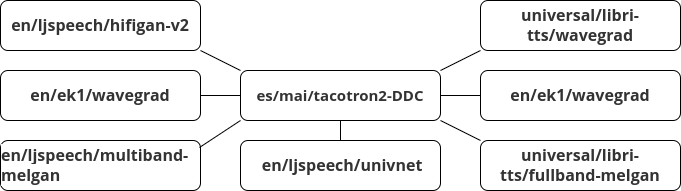
\includegraphics[width=0.7\linewidth]{Graphics/es_mai}
	\caption{Modelo TTS Tacotron2-DDC entrenado en Español}
	\label{esmai}
\end{figure}

\begin{figure}[H]
	\centering
	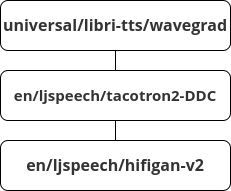
\includegraphics[width=0.3\linewidth]{Graphics/en_ljspeech}
	\caption{Modelo TTS Tacotron2-DDC entrenado en Inglés}
	\label{fig:enljspeech}
\end{figure}

\begin{figure}[H]
	\centering
	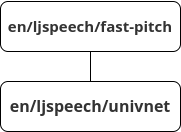
\includegraphics[width=0.3\linewidth]{Graphics/fastpitch}
	\caption{Modelo TTS Fast-Pitch entrenado en Inglés}
	\label{fig:fastpitch}
\end{figure}
\begin{figure}[H]
	\centering
	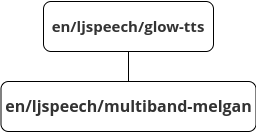
\includegraphics[width=0.4\linewidth]{Graphics/glow_tts}
	\caption{Modelo TTS Glow-TTS entrenado en Inglés}
	\label{fig:glowtts}
\end{figure}


Los modelos \textbf{Tacotron2-DDC, Fast-pitch y Glow-tts} preentrenados en idioma inglés al combinarse con VoCoders, como se observa en las figuras(citar figuras) para un texto en español arroja distintos resultados, en algunos casos solo producen ruido mientras que los más satisfactorios, producen un discurso con una pronunciación propia de una persona de habla inglesa hablando español.

Por otro lado Coqui solo cuenta con un modelo preentrenado en español, el \textbf{Tacontron-DDC}, que está entrenado sobre la base de datos de M-AILABS[\cite{mailabs}]; este modelo fue probado junto a los VoCoders preentrenados como se muestra en la figura \ref{esmai}. Los mejores resultados fueron arrojados por las combinaciones de \textbf{Tacontron-DDC} con los modelos: Univnet entrenado sobre la base de datos Ljspeech en inglés, y Wavegrad entrenado sobre el conjunto de datos LibriTTS, aunque ambos presentan problemáticas como la mala pronunciación de la letra ñ.\\

De acuerdo con la documentación de Coqui, y con el objetivo de la investigación que consiste en desarrollar un sintetizador de voz en español con voz cubana, se consideraron tres enfoques:

\begin{enumerate}
	\item Realizar un \textit{fine-tuning} o reentrenamiento a un modelo preentrenado de [\cite{coqui-doc}], en este caso \textbf{Tacontron-DDC}, que es el único disponible en español. 
	
	\item Realizar el entrenamiendo desde cero de un modelo; en este caso se podría entrenar cualquier modelo disponible. \textbf{Glow-TTS y VITS} son buenos candidatos pues en general producen resultados bastante satisfactorios.% Una desventaja es que cae una gran responsabilidad sobre el conjunto de datos de entrenamiento, pues debe tener una gran riqueza y muchos clips de audio.
	
	\item La problemática del tamaño de la base de datos puede resolverse entrenando el modelo \textbf{YourTTS}, que según la literatura, es capaz de adaptarse a una nueva voz con muy poco tiempo de audio.
\end{enumerate}

Para el desarrollo de cualquiera de los anteriores es imprescindible la construcción de un conjunto de datos que se adapten al modelo y a las necesidades de la investigación.


\section{Creación de la base de datos [\cite{formatting-dataset}]}

Para entrenar un modelo TTS, se necesita un conjunto de datos con grabaciones de voz y transcripciones, en este caso fue una base de datos en español con voces cubanas. El discurso debe dividirse en clips de audio y cada clip necesita su transcripción correspondiente. Debe poseer un formato específico de forma tal que el cargador de datos de Coqui TTS sea capaz de cargarlos para utilizar en el entrenamiento.    

La base de datos conformanda debe tener una buena cobertura del idioma en el que se desea entrenar el modelo. Debe cubrir la variedad fonémica, los sonidos excepcionales y las sílabas. 

\subsubsection{Qué hace a un buen Dataset?}

\begin{itemize}
	\item Debe cubrir una cantidad considerable de clips cortos y largos.
	\item Libre de errores. Se debe eliminar cualquier archivo incorrecto o roto. 
	\item Para escuchar una voz con la mayor naturalidad posible con todas las diferencias de frecuencia y tono, por ejemplo, usando diferentes signos de puntuación.
	\item Es necesario que el \textit{dataset} cubra una buena parte de fonemas, difonemas y, en algunos idiomas, trifonemas. Si la cobertura de fonemas es baja, el modelo puede tener dificultades para pronunciar nuevas palabras difíciles.
	
\end{itemize}

Los clips de audio poseen formato .wav y se organizan dentro de una carpeta de nombre \textit{wavs} de la siguiente forma:

\begin{center}
	/wavs\\
	| - audio1.wav\\
	| - audio1.wav\\
	| - audio2.wav\\
	| - audio3.wav\\
	...
\end{center}

Las transcripciones se recogen dentro del archivo metadata.csv. Donde audio1, audio2, etc se refieren a los archivos audio1.wav, audio2.wav etc.

\begin{center}
	audio1|Esta es mi transcripción 1.
	
	audio2|Esta es mi transcripción 2.
	
	audio3|Esta es mi transcripción 3.
	
	audio4|Esta es mi transcripción 4.
\end{center}

El modelo sobre el que realizaremos el ajuste, está preentrenado sobre la base de datos en Español de \textit{The M-AiLabs Speech Dataset}, por tanto utilizaremos la misma estructura de este en la conformación de la base de datos con voces cubanas. Finalmente queda la siguiente estructura:

\begin{flushleft}
	MyDataset/by$\_$book/female/[creador del dataset]/[nombre del hablante]
	
	|/wavs
	
	|metadata.csv
\end{flushleft}

\section{Reentrenamiendo para el ajuste de Tacontron-DDC}

Se propone desarrollar el primer enfoque: reentrenando(\textit{fine-tuning} en inglés) el modelo \textbf{Tacontron-DDC} en español, pues trae ventajas tales como un aprendizaje más rápido, ya que un modelo preentrenado ya tiene aprendidas funcionalidades que son relevantes para la tarea de producir un discurso. Convergerá más rápido en el nuevo \textit{dataset}, lo que reducirá el costo de entrenamiento y permitirá el proceso de experimentación más rápidamente. Además se pueden obtener buenos resultados con un conjunto de datos más pequeño.  \\

Luego de tener entrenado el modelo acústico(tts) con una base de datos construida con voces cubanas, es posible que alguno de los VoCoders preentrenados disponibles produzca una salida con las características deseadas, en caso contrario se debería entrenar el VoCoder con los datos del \textit{dataset} construido.

\subsection{Fine-Tuning}
Entrenar correctamente un modelo de aprendizaje profundo requiere generalmente de una gran base de datos y de un extenso entrenamiento.

Si se dispone del material necesario y del tiempo para entrenar el algoritmo, estos requisitos no suponen ningún problema, pero, si la base de datos es pequeña o el modelo no se entrena lo suficiente, el aprendizaje podría no ser completo.

El \textit{fine-tuning} es una forma de transferencia de aprendizaje, consiste en aprovechar la información que se ha aprendido de
la resolución de un problema y utilizarla sobre otro distinto, pero que comparte ciertas características. Se usan los conocimientos adquiridos por una red convolucional para transmitirlos a una nueva red convolucional. Esta nueva red convolucional que se crea no tiene por qué modificar la red original y puede simplemente aprender de ella, sin embargo también es válido el caso donde no solo se modifica la red original, sino que se vuelve a entrenar para aprender más conceptos.
  
En la presente investigación, se utiliza el reentrenamiento, para a partir modelo previamente entrenado y realizar un nuevo entrenamientor para mejorar su rendimiento en un conjunto de datos diferente.\\

El proceso consiste en modificar la configuración original del modelo preentrenado seleccionado, es decir, establecer la base de datos a utilizar en el reentrenamiento, los detalles acústicos que reflejen las características del nuevo conjunto de datos, el nombre del nuevo modelo ajustado, la dirección donde se guardará el modelo reentrenado, entre otras cuestiones. Para la mayoría de los parámetros se tomaron las características del modelo original \textbf{Tacontron-DDC} en español.



\section{Entrenamiento de modelo VITS desde cero}

Existen varios modelos de texto a voz de extremo a extremo que permiten el entrenamiento en una sola etapa y el muestreo en paralelo, sin embargo, generalmente la calidad de la muestra no coincide con la de los sistemas TTS de dos etapas. 

Se selecciona VITS porque es un método TTS paralelo de extremo a extremo que genera un sonido de audio más natural que los modelos actuales de dos etapas. Y de acuerdo a una evaluación humana subjetiva (puntuación de opinión media, o MOS), muestra que el modelo supera a los mejores sistemas TTS disponibles públicamente y logra un MOS comparable a la realidad del terreno.


	
	

%Are 100 audio samples sufficient?
%What should be the appropriate learning rate?
%What is the recommended length (no of characters) of each audio sample?
%Should we make any changes to batch size and number of epochs also? (Currently defaults in config file are 64 and 1000 respectively)
%Any other changes which should be done in the config.json file?
%Is tts_models--en--ljspeech--tacotron2-DDC_ph a good model to fine tune for custom voice?







\chapter{Experimentación y Resultados}\label{chapter:implementation}

\section{Instalación de la biblioteca Coqui}
Coqui [\cite{coqui-doc}] es un repositorio de código abierto que implementa las últimas investigaciones en materia de síntesis de voz, como Tacotron 2 y VITS que son los modelos base utilizados en el presente proyecto. Este repositorio ha sido usado para generar modelos en más de 20 idiomas  y cuenta además con múltiples ``recetas'' para el entrenamiento de modelos. 

La biblioteca se instala de acuerdo a las instrucciones orientadas a desarrolladores en [\cite{coqui-doc}].
Con esto ya es suficiente para probar los modelos preentrenados disponibles de Coqui.

\section{Configuración de la evaluación de los modelos} \label{eval}
Se utiliza la medida MOS para la evaluación de los modelos obtenidos en este trabajo. Un puntaje de opinión promedio[\cite{mos}][\cite{mos1}] (MOS, del inglés \textit{Mean Opinion Score}) es una medida numérica de la calidad general de un evento o experiencia juzgada por humanos. En telecomunicaciones, MOS es terminología para clasificación de calidad de audio y video, se refiere a la calidad de escuchar, hablar o conversar, ya sea que se originen en modelos subjetivos u objetivos. Y se evalua de la siguiente forma:
 
  \begin{longtable} [c] { | c | c | }
	\hline
	\endfirsthead
\hline
\endhead
\hline
\endfoot
\hline
\endlastfoot
Muy bueno & 4.3 - 5.0 \\
Malo & 3.1 - 3.6 \\
No recomendado &  2.5 - 3.1\\
Muy malo & 1.0 - 2.5
\label {longtable:1}
\end{longtable}

Debido a la tendencia humana a evitar calificaciones perfectas, entre 4.3 y 4.5 se considera un objetivo de excelente calidad. En el extremo inferior, la calidad del audio o el video se vuelve inaceptable por debajo de un MOS de aproximadamente 3.5. \\

Se utilizaron para la evaluación un total de 6 clips de audio obtenidos de un hablante real, y que expresan las siguientes frases:
\begin{enumerate}
	\item Mis secretos obstáculos, mi miedo inconfesado al baile de máscaras, no se habían aminorado con el cine y sus estímulos, sino que habían crecido de un modo desagradable, y yo, pensando en Armanda, hube de hacer un esfuerzo. \label{sentence1}
	\item Ya tengo de ti la sospecha de que tomas el amor terriblemente en serio. \label{sentence2}
	\item Y, al fin y al cabo, todo lo que él quería era exactamente eso: conocer mundos nuevos. \label{sentence3}
	\item Descubrí a un extraordinario muchachito que me observaba gravemente. Ahí tienen el mejor retrato que más tarde logré hacer de él. La culpa no es mía, las personas mayores me desanimaron cuando sólo había aprendido a dibujar boas cerradas y boas abiertas. \label{sentence4}
	\item Cuando yo tenía seis años vi en el libro sobre la selva virgen: Historias vividas, una grandiosa estampa.Representaba una serpiente boa comiéndose a una fiera. \label{sentence5}
	\item Pido perdón a los niños por haber dedicado este libro a una persona mayor. Tengo una muy seria disculpa: esta persona mayor es el mejor amigo que tengo en el mundo. \label{sentence6}
\end{enumerate}

Se seleccionan estas señales por presentar rasgos característicos del idioma español y que se deben evaluar para arribar a una opinión acerca de si el discurso producido por un modelo en cuestión cumple con el objetivo de la investigación, principalmente en la pronunciación de tildes, y palabras con ñ, además de signos de puntuación. 

La evaluación será conducida por un grupo de expertos del grupo CENATAV, que brindarán una puntuación de 1 a 5 para cada frase de muestra. Finalmente el promedio de estas puntuaciones será reflejado como resultado para cada modelo.  



\subsection{Procesamiento de audio}

\textbf{RNNoise} es una biblioteca basada en una red neuronal para la eliminación de ruido en grabaciones, se utiliza en este proyecto para obtener clips de audio libres de ruidos y con la frecuencia de muestreo deseada.

Se realizó un procesamiento para la eliminación de ruido en el audio de la base de voces original, y se estableció una frecuencia de muestreo de acuerdo a las necesidades de cada experimento. 

\section{Herramientas}
\subsection{Google Colab}
Colaboratory, o Colab[\cite{colab}] para abreviar, es un producto de Google Research, que permite que cualquier persona escriba y ejecute código Python arbitrario a través del navegador y es especialmente adecuado para el aprendizaje automático, el análisis de datos y la educación. Más técnicamente, Colab es un servicio de notebook Jupyter que no requiere configuración para su uso, al tiempo que brinda acceso gratuito a los recursos informáticos, incluidas las GPU. Los recursos de Colab no están garantizados ni son ilimitados, y los límites de uso a veces fluctúan. Esta herramienta fue utilizada para el entrenamiento de modelos durante la investigación, y fue imprescindible el acceso a una suscripción de pago de Colab Pro y la compra de una gran cantidad de recursos. 

\subsection{Google Drive}
Google Drive[\cite{drive}] es un espacio de almacenamiento que permite a los usuarios con cuenta de Google mantener archivos en la nube, y poder compartirlos entre sus distintos dispositivos. La encomienda de Drive en este trabajo fue almacenar las bases de datos utilizadas para los entrenamientos, así como los modelos y archivos de configuración e información que se generan a partir del entrenamiento de una red neuronal profunda con las características de las DNN utilizadas en esta investigación.

\subsection{Espeak phonemizer}
\textbf{Espeak}[\cite{espeak}] es un \textit{software} de texto a voz que admite muchos idiomas y  es compatible con la salida IPA por sus siglas en inglés (\textit{International Phonetic Alphabet}(alfabeto fonético internacional).
El phonemizer permite la fonemización simple de palabras y textos en muchos lenguajes.

\section{Modificación en el código fuente de Coqui TTS} \label{mailabs}
El código fuente del repositorio ocasionaba problemas al conformar ruta del archivo metadata.csv, por lo que se realizó un pequeño cambio en el método \texttt{mailabs} del archivo \texttt{formatter.py}, quedando como se muestra en el siguiente código.


\lstset{language=Python}
\lstset{frame=lines}
\lstset{caption={C\'odigo modificado formatter mailabs}}
\lstset{label={lst:code_direct}}
\lstset{basicstyle=\footnotesize}
\begin{lstlisting}
def mailabs(root_path, meta_files=None, ignored_speakers=None):
"""Normalizes M-AI-Labs meta data files to TTS format

Args:
root_path (str): root folder of the MAILAB language folder.
meta_files (str):  list of meta files to be used in the training. If None, finds all the csv files
recursively. Defaults to None
"""
speaker_regex = re.compile("by_book/(male|female)/(?P<speaker_name>[^/]+)/")
if not meta_files:
csv_files = glob(root_path + "/**/metadata.csv", recursive=True)
else:
csv_files = meta_files

items = []
print(f"{csv_files}")
for csv_file in [csv_files]:
if os.path.isfile(csv_file):
txt_file = csv_file
else:
txt_file = os.path.join(root_path, csv_file)


folder = os.path.dirname(txt_file)
# determine speaker based on folder structure...
speaker_name_match = speaker_regex.search(txt_file)
if speaker_name_match is None:
continue
speaker_name = speaker_name_match.group("speaker_name")
# ignore speakers
if isinstance(ignored_speakers, list):
if speaker_name in ignored_speakers:
continue
print(" | > {}".format(csv_file))
with open(txt_file, "r", encoding="utf-8") as ttf:
for line in ttf:
cols = line.split("|")
if not meta_files:
wav_file = os.path.join(folder, "wavs", cols[0] + ".wav")
else:
wav_file = os.path.join(root_path, folder.replace("metadata.csv", ""), "wavs", cols[0] + ".wav")

if os.path.isfile(wav_file):
text = cols[1].strip()
items.append(
{"text": text, "audio_file": wav_file, "speaker_name": speaker_name, "root_path": root_path}
)
else:
# M-AI-Labs have some missing samples, so just print the warning
print("> File %s does not exist!" % (wav_file))
return items
\end{lstlisting}

\section{Fine-Tuning de Tacontron-DDC} \label{tacotron2}
Como ya se mencionó en el capítulo \ref{chapter:proposal}, el \textit{fine-tuning} resulta una idea prometedora, pues en teoría salva tiempo y recursos.

Para el proceso de ajuste de Tacotron2 a la base de datos personalizada, se utilizó la configuración del modelo preentrenado en español sobre el conjunto de datos de M-AILABS. 

La frecuencia de muestreo(\textit{sample rate}) que se establece en la configuración es 16000Hz, pues el conjunto de datos de M-AILABS sobre el que se preentrenó el modelo seleccionado, se encuentra en esta misma frecuencia. Finalmente se debe utilizar un cargador de datos(\textit{formatter}) compatible con la base de datos usada, en este caso se selecciona la variante \texttt{mailabs}, que se puede apreciar en la sección \ref{mailabs}.

El próximo paso es descargar el modelo Tacotron2, para luego comenzar el reentrenamiento.\\

\texttt{tts - -model$\_$name tts$\_$models$/$es$/$mai$/$tacotron2-DDC - -text "Hola."}\\

\texttt{> Downloading model to $/$home$/$ubuntu$/$.local$/$share$/$tts$/$tts$\_$models--en--ljspeech
	--glow-tts}\\

El reentrenamiento se llevó a cabo utilizando el GPU Premium de Google Colab, y CUDA[\cite{cuda}][\cite{cuda1}]. Requirió una gran cantidad de memoria RAM, siendo 25GB una cantidad insuficiente, se comprobó que con un procesador de 83GB de RAM, sí podía realizarse. El reentrenamiento fue extremandamente costoso, en tiempo y en \textit{computer units}\footnote{Una unidad de cómputo (CU) es la unidad de medida de los recursos consumidos por ejecuciones y compilaciones de actores.}, consumiendo más de 1000CU

Los resultados son extremadamente lastimosos, el modelo entrenado por unas 160 \textit{epochs} produce una señal ruidosa, sin embargo en algún momento se puede distinguir alguna que otra sílaba. A partir de las 210 \textit{epochs} la salida del audio producida para una oración pequeña, es una señal corrupta donde no se distingue nada, este comportamiento se mantienen invariante hasta la \textit{epoch} 580. Se tenía previsto alcanzar las 2000 \textit{epochs}, pero debido a que el reentrenamiento consumía demasiados recursos y visto que los resultados no eran los deseados, no se continuó. 

Claramente el modelo Tacotron2 no se adapta a las necesidades de la investigación, ni a las características de la base de voces conformada, y no cumplió las expectativas de ser un reentrenamiento veloz que iba a converger rápidamente en el nuevo conjunto por estar preentrenado en español. Y es por esto que se decide cambiar a otra DNN.


\section{Entrenamiento de modelo VITS desde cero} \label{vits_s}
Como los resultados de Tacotron2 no fueron los mejores, se optó por realizar experimentos con otros modelos, se eligió VITS por ser de los que mejores resultados arroja por encima de Tacotron2 y Glow-TTS[\cite{kim2021conditional}].

Esta vez se entrena el modelo desde cero utilizando el conjunto de datos con voces cubanas, y la receta[\cite{train-vits}] que provee Coqui[\cite{coqui-doc}] para entrenar VITS. Para este entrenamiento, siguiendo ejemplos de entrenamientos anteriores, se cambia la frecuencia de muestreo de las grabaciones a 22050Hz. Por otro lado el \textit{formatter} utilizado es la variante \texttt{mailabs}, que se encuentra en \texttt{formatters.py}

El entrenamiento se produjo utilizando el GPU Premium de Google Colab, y CUDA[\cite{cuda}][\cite{cuda1}]. Requirió mucha memoria RAM, siendo 25GB una cantidad insuficiente, se comprobó que con un procesador de 83GB de RAM, sí podía realizarse. Transcurrió completa e ininterrumpidamente por 2000 \textit{epochs}, resultando en que el último mejor modelo se generó en la \textit{epoch} número 967. El entrenamiento no representó un gran costo, en tiempo y en \textit{computer units}, demorando alrededor de 7 horas y consumiendo alrededor de 200CU.

Se obtiene un modelo que permite la emisión de sonidos comprensibles, aunque no completamente inteligibles, pues produce un discurso robótico y tiene dificultad en la combinación de difonos, por lo que hay frases y palabras indescifrables para el oyente.

Finalmente se sometió el modelo, al proceso de evaluación descrito en la sección \ref{eval} con la medida MOS, arrojando los siguientes resultados:

\begin{center} \begin{tabular}{ |c|c|c| } 
\hline 
Muestra & Puntuación \\
\hline
frase \ref{sentence1} & 2.5 \\
frase \ref{sentence2} & 2.0 \\
frase \ref{sentence3} & 2.5 \\
frase \ref{sentence4} & 1.0 \\
frase \ref{sentence5} & 1.0 \\
frase \ref{sentence6} & 1.0 \\
\hline
Medida MOS & 1.6\\
 \hline 
\end{tabular} 
\end{center}

Se demuestra que el entrenamiento del modelo VITS desde cero con los datos descritos, es desalentador.


\section{Fine-tuning de modelos VITS preentrenados} \label{vits_it_en}

\subsection{Modelo preentrenado en italiano}
El modelo disponible de Coqui en idioma italiano fue preentrenado sobre la base de datos en italiano de M-AILABS, cuyas grabaciones poseen una frecuencia de muestreo de 16000Hz, por tanto la base de voces cubanas que se utiliza para el \textit{fine-tuning} fue llevado a la misma frecuencia.
El \textit{formatter} utilizado es igualmente la variante \texttt{mailabs}.

El proceso de \textit{fine-tuning} se llevó a cabo utilizando el GPU Premium de Google Colab, y CUDA[\cite{cuda}][\cite{cuda1}]. Requirió una gran cantidad de memoria RAM, siendo 25GB una cantidad insuficiente, no se precisa exactamente la cantidad de RAM necesaria, sin embargo, se comprobó que con un procesador de 83GB de RAM, sí podía realizarse sin problemas. Además de esto, no representó un gran costo, en tiempo y en \textit{computer units}, demorando alrededor de 3 horas y consumiendo alrededor de 40CU.

El modelo que se genera luego de un reentrenamiento ininterrumpido durante 1000 \textit{epochs}, arroja como resultado que, para una frase escrita dada, produce un discurso bastante comprensible, aunque un poco robótico, y entrecortado en alguna partes. Además con palabras que el oyente no puede descifrar. Es importante destacar que el modelo original de Coqui en italiano produce también una voz ruidosa, así que la cuestión del ruido es probable que venga desde el modelo inicial, agravada con el \textit{fine-tuning} a partir del \textit{Cuban Voice Dataset}.

Por último se realiza el proceso de evaluación descrito en la sección \ref{eval} con la medida MOS, arrojando los siguientes resultados:

\begin{center} \begin{tabular}{ |c|c|c| } 
		\hline 
		Muestra & Puntuación \\
		\hline
		frase \ref{sentence1} & 3.0 \\
		frase \ref{sentence2} & 2.7 \\
		frase \ref{sentence3} & 2.6 \\
		frase \ref{sentence4} & 2.2 \\
		frase \ref{sentence5} & 2.1 \\
		frase \ref{sentence6} & 2.3 \\
		\hline
		Medida MOS & 2.4\\
		\hline 
	\end{tabular} 
\end{center}

Se evidencia una mejora en los resultados, con respecto al modelo anterior. Esto es debido a que el modelo ya tenía aprendidas características del idioma italiano, que es uno de los más similares al español.


\subsection{Modelo preentrenado en Inglés} 
La variante del modelo VITS entrenada sobre el conjunto LJ-Speech Dataset[\cite{ljspeech}] en inglés, se seleccionó por ser el inglés un idioma, más distante del español que el italiano. Se lleva a cabo el mismo proceso que en el caso anterior, con la diferencia de que la base de datos \textit{Cuban Voice Dataset} cambia su frecuencia de muestreo a 22050Hz. 
El reentrenamiento se realizó siguiendo las mismas características que en el modelo en italiano, y consumió alrededor del mismo tiempo y recursos.

Por último el modelo en inglés ajustado a la base de datos cubana arroja resultados diferentes al modelo que se obtiene a partir del modelo italiano. Un aspecto a favor es que el ruido, y la pronunciación robótica no están presentes en el nuevo discurso, y la voz sintética suena bastante parecida a la del hablante, un objetivo que hasta este punto no había sido alcanzado. Sin embargo, y como era de esperar, gramatical y fonéticamente presenta más problemas, entre ellos la pronunciación de la ñ y las r unidas a vocales, entre otros bastante evidentes al escuchar la salida de audio.

Se realiza el proceso de evaluación descrito en la sección \ref{eval} con la medida MOS, arrojando los siguientes resultados:

\begin{center} \begin{tabular}{ |c|c|c| } 
		\hline 
		Muestra & Puntuación \\
		\hline
		frase \ref{sentence1} & 1.5 \\
		frase \ref{sentence2} & 2.7 \\
		frase \ref{sentence3} & 3.7 \\
		frase \ref{sentence4} & 2.0 \\
		frase \ref{sentence5} & 1.9 \\
		frase \ref{sentence6} & 2.2 \\
		\hline
		Medida MOS & 2.3\\
		\hline 
	\end{tabular} 
\end{center}

Los resultados son ligeramente peores que con el \textit{fine-tuning} del modelo preentrenado en italiano. No resulta una gran sorpresa pues el inglés es un idioma más distante al español.

\section{Entrenamiento con M-AILABS DATASET} \label{vits_angel}
Se comienza a sospechar, que probablemente la base de datos \textit{Cuban Voice Dataset} no cuente con la riqueza necesaria para que un modelo realice un aprendizaje adecuado que reporte resultados aceptables. Debido a esto se considera la idea de realizar un entrenamiento desde cero sobre modelo VITS utilizando el conjunto de datos de \textit{The M-AILABS Dataset} con su única voz femenina Angelina, este conjunto cuenta con más de 7000 clips de audio para el entrenamiento, con un \textit{sample rate} de 16000Hz.

El entrenamiento se realiza nuevamente en Google Colab, con las mismas características de los anteriores, aunque, esta vez por la densidad de la base de datos el proceso demora más, tomando alrededor de 12 horas para llegar a 321 \textit{epochs}, y consumiendo una cantidad proporcional de recursos.

El modelo que se obtiene produce una señal inteligible y libre de ruidos, aunque mejorable en algunas expresiones, pues la meta ideal sería un entrenamiento de 1000 \textit{epochs}.

Con un modelo que arroja resultados bastante buenos, se procede a realizar \textit{fine-tuning} sobre la base de datos obtenida de la investigación, se efectúa con la misma configuración que el entrenamiento anterior, por alrededor de 1000 \textit{epochs}, y arroja los mejores resultados obtenidos sobre este conjunto de datos. Sin embargo, tampoco se consideran buenos, pues aunque se elimina el ruido en las grabaciones, muchas palabras resultan aún indescifrables para el oyente.

A continuación las evaluaciones de expertos utilizando la medida MOS:


\begin{table}[H]
	\begin{center} 
\begin{tabular}{ |c|c| } 
	\hline
	Muestra & Puntuación \\
	\hline
	frase \ref{sentence1} & 4.3 \\
	frase \ref{sentence2} & 4.4 \\
	frase \ref{sentence3} & 4.4 \\
	frase \ref{sentence4} & 4.3 \\
	frase \ref{sentence5} & 4.3 \\
	frase \ref{sentence6} & 4.4 \\
	\hline
	Medida MOS & 4.35\\
	\hline
\end{tabular}
\caption{Resultados de modelo VITS entrenado desde cero con la base de datos de M-AILABS} 
\end{center}
\end{table}
	
\begin{table}[H]
	\begin{center} 
		\begin{tabular}{ |c|c| } 
			\hline
			Muestra & Puntuación \\
			\hline
			frase \ref{sentence1} & 2.5 \\
			frase \ref{sentence2} & 2.8 \\
			frase \ref{sentence3} & 4.1 \\
			frase \ref{sentence4} & 3.6 \\
			frase \ref{sentence5} & 2.3 \\
			frase \ref{sentence6} & 3.5 \\
			\hline
			Medida MOS & 3.1\\
			\hline
		\end{tabular}
		\caption{Resultados del fine-tuning al modelo VITS entrenado desde cero con la base de datos de M-AILABS} 
	\end{center}
\end{table}

Las mejores puntuaciones las recibe el modelo entrenado con la base de datos fuente, \textit{The M-AILABS Dataset}[\cite{mailabs}], de aquí la importancia del conjunto de datos para el entrenamiento de modelos.\\

\section{Conclusiones Parciales}

A raíz de los resultados obtenidos en las secciones \ref{tacotron2}, \ref{vits_s}, \ref{vits_it_en}, \ref{vits_angel} es posible concluir que Tacotron2 parece ser una red demasiado grande que no se adapta a las necesidades de la investigación, produciendo finalmente señales corruptas e indescifrables.

El modelo VITS es significativamente mejor en lo que respecta a la velocidad del entrenamiento, y además más adaptable a nuevos conjuntos de datos. Con un entrenamiento desde cero sobre una base de datos relativamente pequeña y rústica, produce un discurso bastante malo, aunque entendible en ocasiones. De forma similar sucede con el modelo VITS preentrenado en italiano y luego sometido a un proceso de \textit{fine-tuning} con el conjunto mencionado anteriormente, a pesar de la rapidez del entrenamiento, produce una señal algo ruidosa, y solo entendible en ocasiones. El mejor resultado con diferencia es el producido por el modelo VITS entrenado desde cero con una base de datos fuerte, aunque este no cumple con el objetivo de la investigación pues la voz corresponde a un hablante mexicano. El discurso obtenido de este modelo recibe la mayor medida MOS. Al mismo tiempo al realizar \textit{fine-tuning} sobre este modelo con la base de datos cubana, el audio empeora y resulta incomprensible en ocasiones. Debe ser aclarado que este último modelo es el mejor resultado obtenido sobre el conjunto de datos conformado con voces cubanas, con la obtención de grabaciones libres de ruido. 






\backmatter

\begin{conclusions}    
Esta investigación presenta como objetivo el desarrollo de un sistema de síntesis de texto a voz en español, que sintetizara una voz con acento cubano. Se realizó un estudio de las tecnologías existentes para realizar la síntesis de voz, arribando a la conclusión que los últimos estudios basados en redes neuronales, eran los más adecuados para este trabajo por ser los que mejores resultados presentaban. Mediante un análisis de los métodos TTS basados en redes neuronales, y las bibliotecas disponibles para este fin, se selecciona Coqui como herramienta base. 

Se comprobó que todos los modelos TTS disponibles en Coqui, necesitan para su entrenamiento una base de datos de audio con sus transcripciones correspondientes. Para cumplir la meta de generar una voz con acento cubano el encargado de esta investigación, construyó una base de datos con un hablante cubano, que contó con 160 clips de audio. En comparación con las bases de datos fuentes disponibles, esta fue relativamente pequeña, pues la construcción de una base de voces es una tarea costosa en tiempo, y la premura de la entrega de la tesis no permitió la creación de una fuente de datos más completa.

Se procedió entonces al reentrenamiento del modelo basado en síntesis neuronal. El modelo VITS se muestra ser la selección correcta luego de realizar experimentos no satisfactorios con el modelo Tacotron2. Se entrenan desde cero y reentrenan un número de 5 modelos VITS, para comprobar los mejores resultados. Finalmente, se evalúa mediante la opinión de expertos la calidad del audio producido por estos modelos, utilizando la medida MOS. Los mejores resultados fueron arrojados por el modelo VITS entrenado desde cero con la base de datos fuente de M-AILABS, sin embargo este no cumple con el requisito del acento cubano. Ninguno de los modelos entrenados con la base de datos con voces cubanas, obtenida como resultado de esta tesis, produjo resultados completamente satisfactiorios, quedando como más aceptable el obtenido mediante el ajuste del modelo entrenado con la base de datos fuente, al conjunto de datos construido para este trabajo.
 
Concluimos que el mayor peso para lograr una síntesis de datos apropiada recae sobre el conjunto de datos para el entrenamiento.

Los anteriores elementos contribuyeron al cumplimiento del objetivo general, dar los primeros pasos hacia el desarrollo de un sintetizador de texto a voz con voces cubanas. 
    
    
   
\end{conclusions}

\begin{recomendations}
    Recomendaciones
\end{recomendations}

\printbibliography[heading=bibintoc]


\end{document}